% Based on the supplied Template_LaTeX/main.tex; see WORD_IMPORT.md.
\documentclass[12pt,reqno, twoside]{amsbook}
%%%%%%%%%%%%%%%%%%%%%%%%%%%%%%%%%%%%%%%%%%%%%%%%%%%%%%%%%%%%%%%%%%%%%%%%%%%%%%%%%%%%%%%%%%%%%%%%%%%%%%%%%%%%%%%%%%%%%%%%%%%%%%%%%%%%%%%%%%%%%%%%%%%%%%%%%%%%%%%%%%%%%%%%%%%%%%%%%%%%%%%%%%%%%%%%%%%%%%%%%%%%%%%%%%%%%%%%%%%%%%%%%%%%%%%%%%%%%%%%%%%%%%%%%%%%
\usepackage{eurosym}
\usepackage{amsmath}
\usepackage{amssymb}
\usepackage{amsfonts}
\usepackage[onehalfspacing]{setspace}
\usepackage{chngcntr}
\usepackage{graphicx}
\usepackage[a4paper, margin=2.5cm]{geometry}
\usepackage[english]{babel}
\usepackage{fancyhdr}
\usepackage{titlesec}
\usepackage{enumitem}
\usepackage{etoolbox}
\usepackage{csquotes}
\usepackage[printonlyused]{acronym}
%
% you may need to uncomment the command below if you use eps format for figures
%\usepackage{epstopdf}
%
\usepackage[
    backend=biber,
    style=ieee,
  ]{biblatex}
\addbibresource{../refs/references.bib}
%
\makeatletter
    \def\section{\@startsection{section}{1}%
      \z@{.5\linespacing\@plus.7\linespacing}{.25\linespacing}%
      {\normalfont\bfseries\flushleft}}
    \def\subsection{\@startsection{subsection}{2}%
      \z@{.5\linespacing\@plus.7\linespacing}{.25\linespacing}%
      {\normalfont\bfseries\flushleft}}
%
\makeatother
\setcounter{MaxMatrixCols}{10}
%
\providecommand{\U}[1]{\protect\rule{.1in}{.1in}}
\theoremstyle{plain}
\newtheorem{acknowledgement}{Acknowledgement}
\newtheorem{algorithm}{Algorithm}[chapter]
\newtheorem{axiom}{Axiom}[chapter]
\newtheorem{case}{Case}[chapter]
\newtheorem{claim}{Claim}[chapter]
\newtheorem{conclusion}{Conclusion}[chapter]
\newtheorem{condition}{Condition}[chapter]
\newtheorem{conjecture}{Conjecture}[chapter]
\newtheorem{corollary}{Corollary}[chapter]
\newtheorem{criterion}{Criterion}[chapter]
\newtheorem{definition}{Definition}[chapter]
\newtheorem{example}{Example}[chapter]
\newtheorem{exercise}{Exercise}[chapter]
\newtheorem{lemma}{Lemma}[chapter]
\newtheorem{notation}{Notation}[chapter]
\newtheorem{problem}{Problem}[chapter]
\newtheorem{proposition}{Proposition}[chapter]
\newtheorem{remark}{Remark}[chapter]
\newtheorem{solution}{Solution}[chapter]
\newtheorem{summary}{Summary}[chapter]
\newtheorem{theorem}{Theorem}[chapter]
\numberwithin{equation}{chapter}
%
\makeatletter
\newcommand\frontFont{\@setfontsize\frontFont{14.4}{14.4}}
\makeatother
%
% Please write the references according to your school
%
\newenvironment{dedication}
  {%\clearpage           % we want a new page
   \thispagestyle{empty}% no header and footer
   \vspace*{\stretch{1}}% some space at the top
   \itshape             % the text is in italics
   \raggedleft          % flush to the right margin
  }
  {\par % end the paragraph
   \vspace{\stretch{3}} % space at bottom is three times that at the top
   %\clearpage           % finish off the page
  }
  \numberwithin{section}{chapter}
\fancyhead{}
\fancyfoot{}
\pagestyle{fancy}
\fancyfoot[LE,RO]{\thepage}
%
\makeatletter
\def\ps@plain{\ps@empty
 \def\@evenfoot{%
   \normalfont\scriptsize
   \rlap{\thepage}\hfil
   }%
 \def\@oddfoot{%
   \normalfont\scriptsize \hfil
   \llap{\thepage}}%
}
\makeatother
\renewcommand{\headrulewidth}{0pt}
\renewcommand{\footrulewidth}{0pt}
%
\usepackage{montserrat}
\usepackage[T1]{fontenc}
\renewcommand*\oldstylenums[1]{{\fontfamily{Montserrat-TOsF}\selectfont #1}}
%
\numberwithin{table}{chapter}
\numberwithin{figure}{chapter}
%
%%% PT: BEGIN
% \addto\captionsenglish{\renewcommand{\chaptername}{Capítulo}}
% \addto\captionsenglish{\renewcommand{\tablename}{Tabela}}
% \addto\captionsenglish{\renewcommand{\figurename}{Figura}}
% \addto\captionsenglish{\renewcommand{\figurename}{Figura}}
% \addto\captionsenglish{\renewcommand{\contentsname}{Conteúdo}}
% \addto\captionsenglish{\renewcommand{\listfigurename}{Lista de Figuras}}
% \addto\captionsenglish{\renewcommand{\listtablename}{Lista de Tabelas}}
% \DeclareDelimFormat{finalnamedelim}{\addspace e\space}
%%% PT: END
%

\newcommand{\thesistitle}{Blockchain-powered Personal AI -- Digital Twin Edge Gateway}

% Typesetting support for the Word source's tables and preserved references.
\usepackage{booktabs,longtable,array,ragged2e}
\newcounter{none}
\usepackage{xurl}
\usepackage{microtype}
\providecommand{\tightlist}{\setlength{\itemsep}{0pt}\setlength{\parskip}{0pt}}
\ExecuteBibliographyOptions{sorting=none}
\DeclareFieldFormat[misc]{note}{#1}
\DeclareBibliographyDriver{misc}{\printfield{note}\finentry}
\setlength{\emergencystretch}{2em}

\begin{document}

\sffamily
\frontFont
\begin{flushleft}
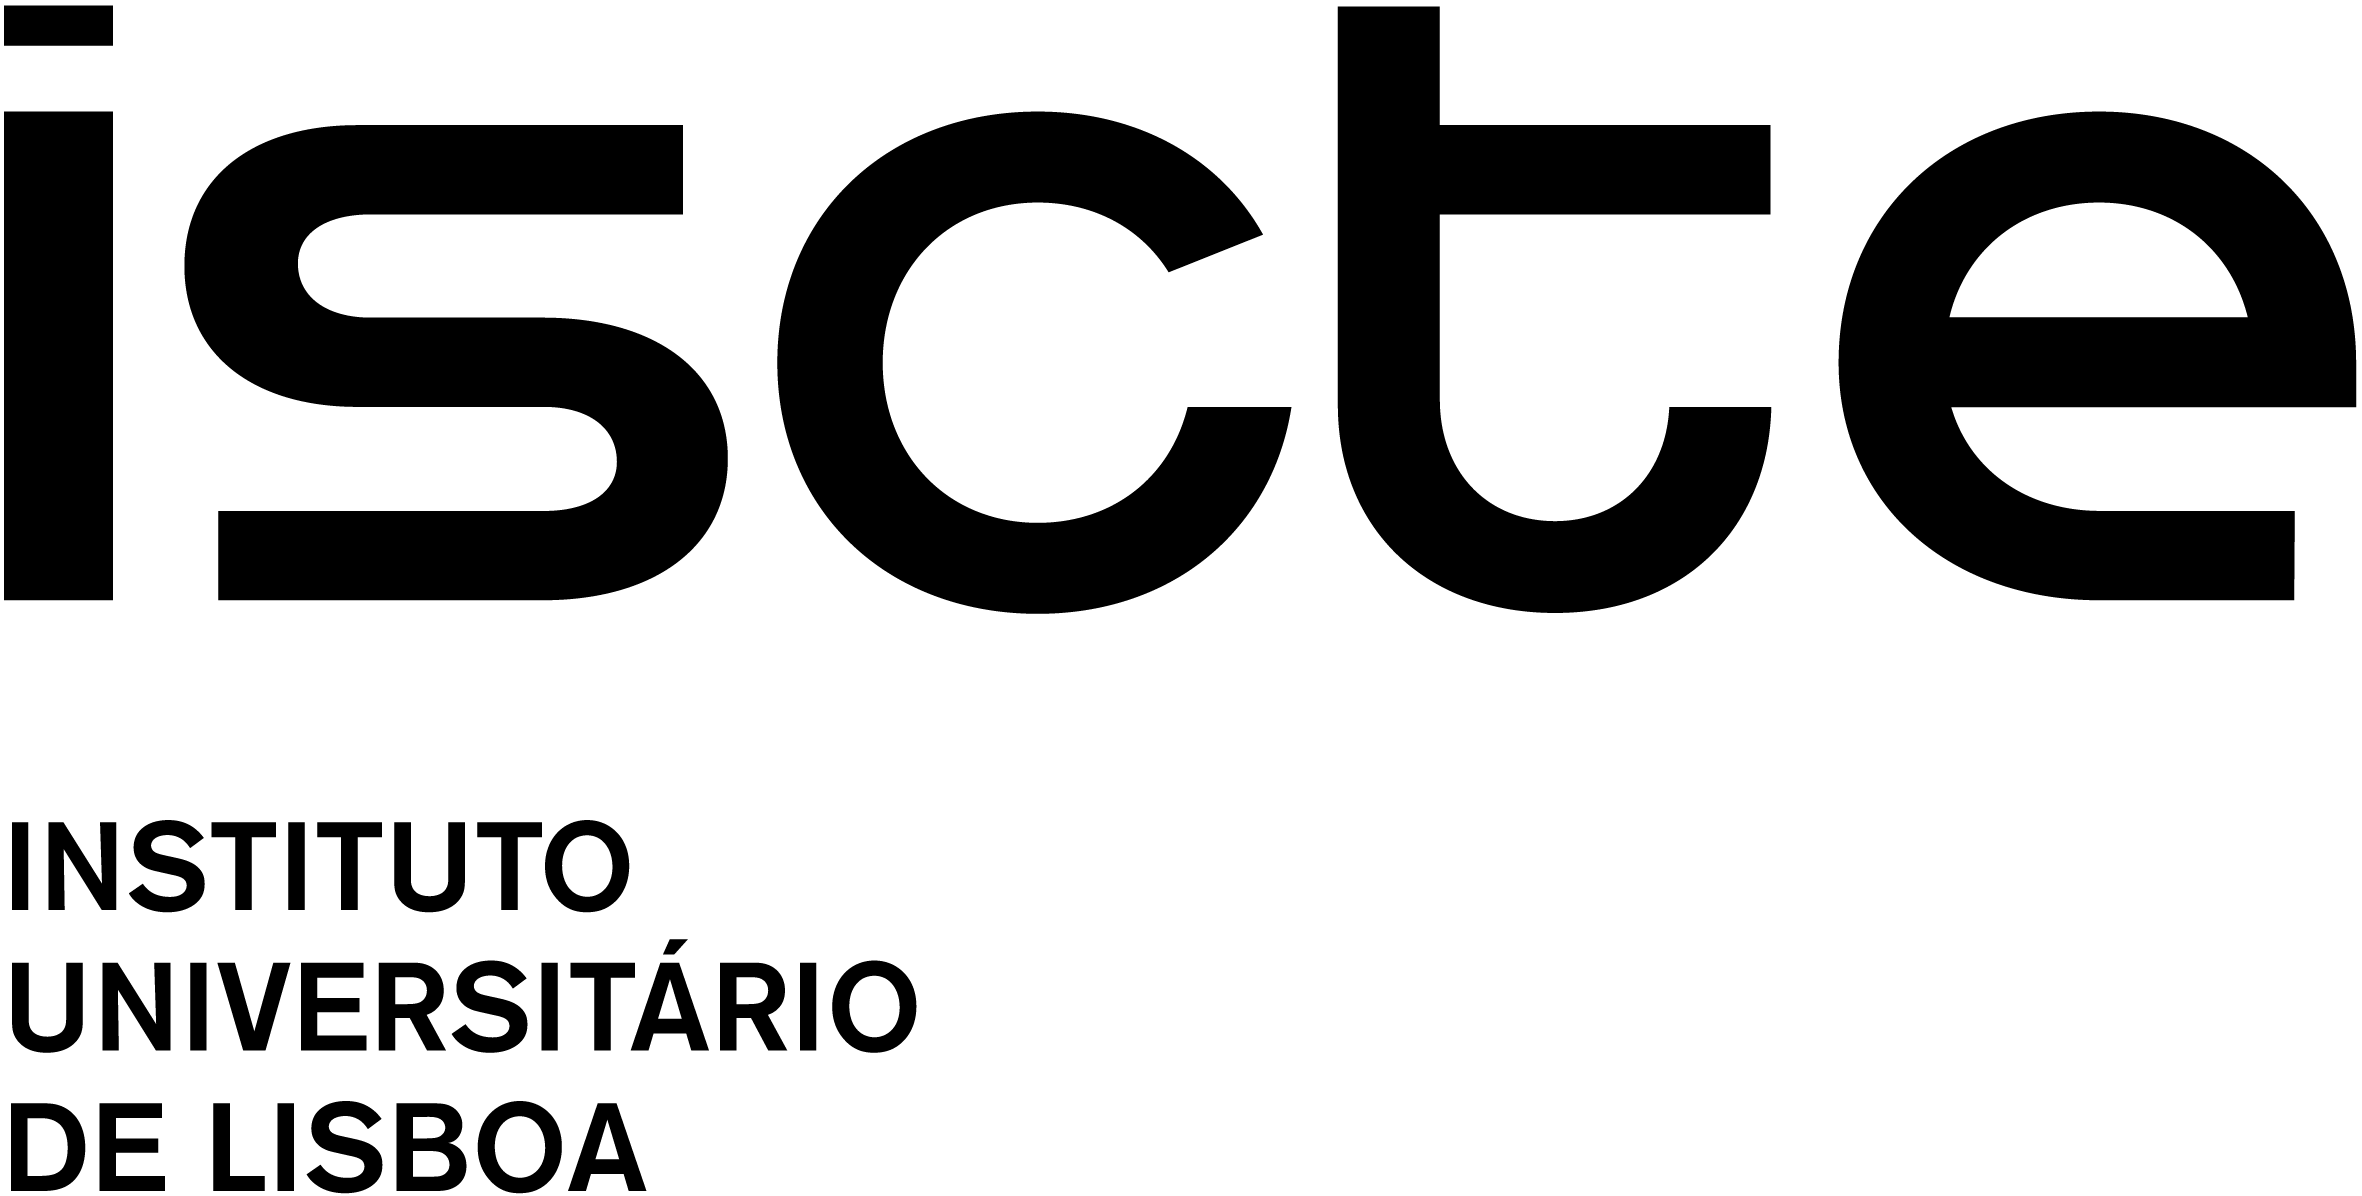
\includegraphics[width=6.03cm]{imagens/iscte}\\[3.3mm]

\hrulefill
~\\
~\\
~\\
\textbf{\thesistitle}\\
~\\
~\\
~\\
\textit{Rui Miguel Franco Duarte}\\
\textit{Student number: 94494}\\
~\\
~\\
~\\
Master in Telecommunications and Computer Engineering\\
~\\
~\\
~\\
Supervisor:\\
\mbox{}\\
Iscte -- Instituto Universitário de Lisboa\\
~\\
~\\
~\\
Co-Supervisor:\\
\mbox{}\\
\mbox{}\\
~\\
~\\
~\\
Lisbon, 2025/2026
\end{flushleft}
\thispagestyle{empty}
\cleardoublepage
\begin{flushleft}
  
\includegraphics[width=6.03cm]{imagens/ista}\\[7mm]
\hrulefill
~\\
~\\
~\\
Department of Information Science and Technology\\
~\\
~\\
\textbf{\thesistitle}\\
~\\
~\\
~\\
\textit{Rui Miguel Franco Duarte}\\
\textit{Student number: 94494}\\
~\\
~\\
~\\
Master in Telecommunications and Computer Engineering\\
~\\
~\\
~\\
Supervisor:\\
\mbox{}\\
Iscte -- Instituto Universitário de Lisboa\\
~\\
~\\
~\\
Co-Supervisor:\\
\mbox{}\\
\mbox{}\\
~\\
~\\
~\\
Lisbon, 2025/2026
  \end{flushleft}
  \thispagestyle{empty}

\rmfamily
\normalsize
\frontmatter
\addtocontents{toc}{\setcounter{tocdepth}{2}}
\begin{dedication}
\end{dedication}
\chapter*{Acknowledgment}
\chapter*{Resumo}
\chapter*{Abstract}
\tableofcontents
\listoffigures
\listoftables
\cleardoublepage
\chapter*{List of Acronyms}
\begingroup\def\LTcaptype{none}
\small\setstretch{1.05}
\begin{longtable}{@{}>{\RaggedRight\arraybackslash}p{\dimexpr 0.12\linewidth-0.72\tabcolsep\relax}>{\RaggedRight\arraybackslash}p{\dimexpr 0.39\linewidth-2.34\tabcolsep\relax}>{\RaggedRight\arraybackslash}p{\dimexpr 0.12\linewidth-0.72\tabcolsep\relax}>{\RaggedRight\arraybackslash}p{\dimexpr 0.37\linewidth-2.2199999999999998\tabcolsep\relax}@{}}
\toprule
AMQP & Advanced Message Queuing Protocol & JSON-LD & JSON for Linked Data \\
\midrule\endfirsthead
\toprule
AMQP & Advanced Message Queuing Protocol & JSON-LD & JSON for Linked Data \\
\midrule\endhead
\bottomrule\endfoot
ARM64 & 64-bit ARM architecture & MQTT & Message Queuing Telemetry Transport \\
\addlinespace[3pt]
BLE & Bluetooth Low Energy & NAT & Network address translation \\
\addlinespace[3pt]
C2DTA & Consumer-Controlled Digital Twin Architecture & OCI & Open Container Initiative \\
\addlinespace[3pt]
DID & Decentralized identifier & QEMU & Quick Emulator \\
\addlinespace[3pt]
DIDComm & DID-based agent-to-agent communication protocol & QoS & Quality of service \\
\addlinespace[3pt]
DSR & Design Science Research & SSI & Self-sovereign identity \\
\addlinespace[3pt]
HTTP & Hypertext Transfer Protocol & TLS & Transport Layer Security \\
\addlinespace[3pt]
IoT & Internet of Things & W3C & World Wide Web Consortium \\
\addlinespace[3pt]
IPFS & InterPlanetary File System & WoT & Web of Things \\
\addlinespace[3pt]
JSON & JavaScript Object Notation &  &  \\
\end{longtable}
\endgroup

\mainmatter
\chapter{Introduction}\label{chapter-1.-introduction}

\section{Background and Motivation}\label{background-and-motivation}

\noindent \emph{Edge computing} places computing and storage nodes at the edge of the Internet, close to the mobile devices and sensors that produce data \cite{word01}, \cite{word02}. Low latency is one of the benefits because cloud data centers are not suitable for applications that need end-to-end delays below a few tens of milliseconds \cite{word01}. Sending every reading to the cloud also spends bandwidth and computing unnecessarily when the edge produces large quantities of data \cite{word02}. Privacy adds an additional reason, because the physical data that devices collect at the edge is usually private, as with wearable health devices\cite{word02}. In the smart home, the gateway is the edge between home devices and the cloud, and most of the data it gathers can stay inside the home\cite{word02}.

Most wearable devices combine personal data with dependence on another device. Most data from wearable sensors are personal and uniquely represents the user and communicate over Bluetooth or Bluetooth Low Energy \cite{word03}. A \emph{digital twin} is a software representation of an individual physical object that remains its virtual counterpart across the object\textquotesingle s lifecycle \cite{word04}. There are three types of digital representation, a digital model has no automatic data exchange, a digital shadow receives a one-way flow from the physical object, and a digital twin exchanges data automatically in both directions \cite{word05}. Whoever hosts the twin of a wearable therefore receives its personal data.

The Consumer-Controlled Digital Twin Architecture (C2DTA) moves the digital twin of a smart device from a manufacturer-controlled cloud to an edge gateway under consumer control \cite{word06}. The gateway hosts the twin platform, and this shift makes consumers the \emph{de facto} controllers of their smart-device data \cite{word06}. In its implementation, Eclipse Ditto manages the twins, and Eclipse Mosquitto carries sensor data, alongside Hyperledger Indy, Aries and Fabric and the InterPlanetary File System \cite{word06}.

In this dissertation, the \emph{local twin core} denotes the message broker, the controller and the twin platform that receive telemetry, validate it and keep twin state on the gateway. Within the sources examined, no evaluation covers a C2DTA-style local twin core on native ARM64 with concurrent telemetry from several wearable types under a pre-specified protocol. This dissertation builds and evaluates one integrated gateway. A versioned Yocto Project image supplies its Linux kernel and root filesystem and boots as the operating system of a native ARM64 virtual machine. On that system, a container stack materializes synthetic smartwatch, smart-ring and smart-clothing telemetry as twins in Eclipse Ditto. The same Yocto layers also produce a Quick Emulator (QEMU) target for functional checks, which run under processor emulation on the build host and yield no performance result.

\section{Research Questions}\label{research-questions}

\noindent The research questions (RQs) address one of the four roles that the C2DTA assigns to its Edge Gateway: hosting the digital-twin platform\cite{word06}. RQ1 covers the versioned gateway image, its deployment and redeployment on an ARM64 virtual machine and the container stack that the image hosts. RQ2 and RQ3 belong to the evaluation of the integrated gateway on that virtual machine.

\begin{quote}
\textbf{RQ1.} How can a version of Yocto-based ARM64 gateway image be built, deployed and redeployed in an ARM64 virtual machine to host the local digital-twin core of C2DTA?

\textbf{RQ2.} To what extent can the integrated gateway ingest and materialize concurrent synthetic telemetry from three wearable-device types correctly and reliably, including under specified fault scenarios?

\textbf{RQ3.} What latency, sustainable-throughput, saturation and per-container resource trade-offs characterize the integrated gateway under controlled loads on the selected ARM64 virtual machine?
\end{quote}

Each question calls for a separate kind of evidence. For RQ1, the evidence comes from identified builds of the image and from its boots on QEMU and on the ARM64 virtual machine. Redeploying the container stack on that machine with digest-pinned Linux/arm64 images completes the evidence. RQ2 depends on a classified outcome for every message in the nominal, dropout-reconnect and invalid-payload scenarios. The load-sweep scenario targets sustainable throughput and saturation for RQ3, while controller-side latency and per-container processor and memory use complete its evidence.

\section{Objectives}\label{objectives}

\noindent The general objective is to design, build and experimentally evaluate an integrated, versioned Yocto-based ARM64 Edge Gateway that hosts the local digital-twin core of C2DTA. Five specific objectives decompose the general objective, two for the gateway and three for the evaluation and its evidence.

\begin{enumerate}
\def\labelenumi{\arabic{enumi}.}
\item
  Build a versioned Yocto Project image, with systemd, networking and a container runtime, that boots on QEMU for functional checks and on a native ARM64 virtual machine.
\item
  Deploy, on the system booted from that image, an ARM64 container stack materializing validated Message Queuing Telemetry Transport (MQTT) messages as digital twins in Eclipse Ditto.
\item
  Implement a command-line simulator for smartwatch, smart ring and smart clothing telemetry.
\item
  Define test scenarios, from smoke test to 24-hour tests, and pre-specify the evaluation protocol of the campaign on the ARM64 virtual machine.
\item
  Assemble a versioned evidence package with code, configurations, logs, data, checksums and the analysis script.
\end{enumerate}

\section{Research Method}\label{research-method}

\noindent This dissertation applies the Design Science Research (DSR) methodology \cite{word07}, whose practice rules require an artefact that addresses a problem and its rigorous evaluation. Its process model has six activities: problem identification and motivation, objectives of a solution, design and development, demonstration, evaluation and communication\cite{word07}. Research may enter this nominal sequence at any of its first four activities\cite{word07}.

This work enters at the first activity, the problem-centered approach \cite{word07} that links to ideas arising from the future research suggested in a prior paper. The C2DTA article is that prior paper, and its evaluation and stated future work supply the idea for this dissertation \cite{word06}. Sections 1.1 and 2.9 set out the problem, Section 1.3 derives the objectives from it, and Section 2.1 gives the literature review method.

Figure 1.1 maps the six activities onto this work, which starts from the problem of Section 1.1. Design and development the ARM64 Yocto image, the container stack and its controller that run on the system booted from that image, and the deterministic telemetry simulator. Demonstration uses the artefact to solve instances of the problem \cite{word07}. In this work it repeats builds and boots of the image, on QEMU and on the ARM64 virtual machine. It also traces one message through the controller into Eclipse Ditto on the integrated gateway. The evaluation compares the observed results with the objectives \cite{word07}, and communication includes this dissertation and the evidence package. Functional gates for build, boot, vertical slice and protocol freeze return the process from demonstration to design.

\begin{figure}[htbp]
\centering
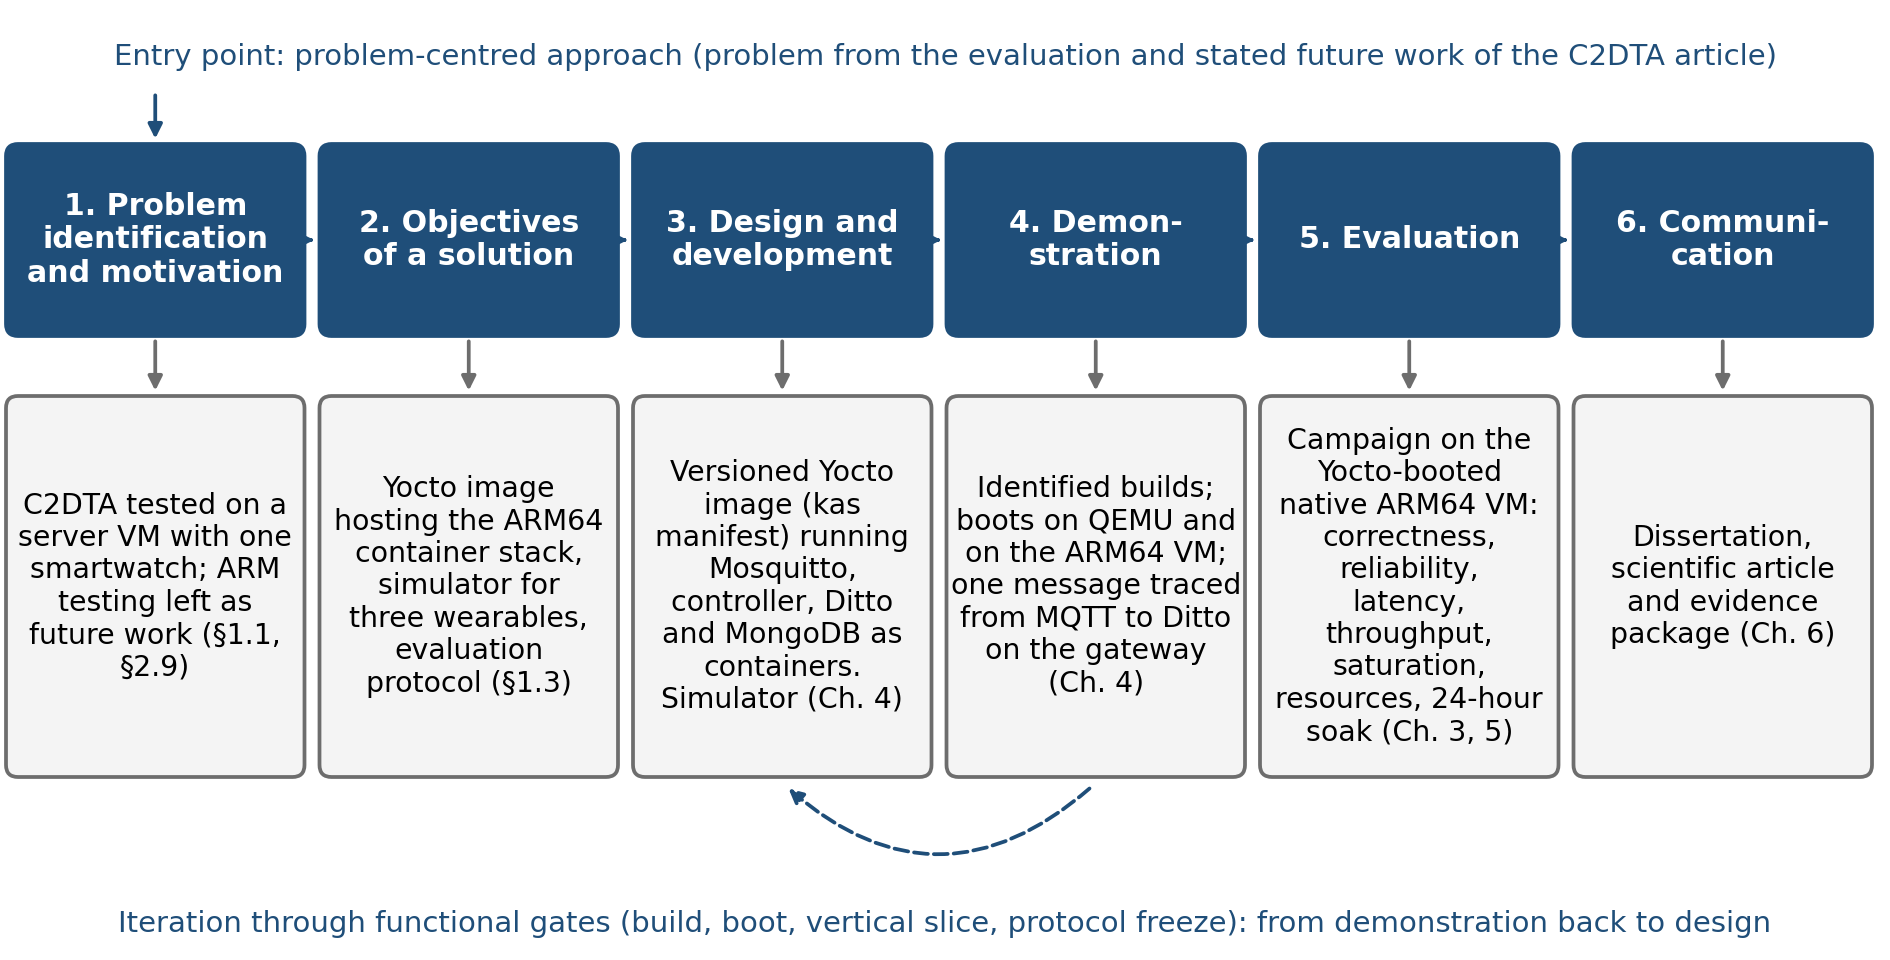
\includegraphics[width=\linewidth]{imagens/research-process.png}
\caption{Research process of this dissertation, instantiating the DSR methodology process model}
\label{fig:research-process}
\end{figure}

The evaluation runs under a pre-specified protocol on a temporary, non-burstable native ARM64 virtual machine that boots the Yocto-built kernel and root filesystem. Emulated boots on QEMU serve functional checks only, and a result on the ARM64 virtual machine characterizes that platform configuration. The run is the statistical unit, and the controller measures latency on a monotonic clock, from reception to the Ditto acknowledgement. Chapter 3 selects the platform and details the protocol and its statistical treatment.

\section{Document Structure}\label{document-structure}

\noindent After this introduction, Chapter 2 sets out the theoretical framework, and Section 2.1 describes the literature review method. The methodology of Chapter 3 selects the evaluation platform and defines the protocol, the scenarios, the metrics with their operational definitions and the statistical treatment. Chapter 4 describes the architecture and implementation: the Yocto image and its targets, the container stack, the message and interface contracts, the simulator and the controller.

The evaluation and its results form Chapter 5. Chapter 6 draws the conclusions and identifies future work.

\chapter{Theoretical Framework}\label{chapter-2.-theoretical-framework}

\section{Literature Review Methodology}\label{literature-review-methodology}

\noindent A structured review with systematic elements grounds Chapter 2 and the artefact\textquotesingle s design decisions in verified literature. Those elements are logged search strings, dated queries, explicit criteria, deduplication, snowballing and metadata verification. The review fits the purpose of mapping evidence across ten axes to ground design decisions, rather than answering one narrow question by exhaustive synthesis.

Table 2.1 lists the ten review axes with their topics and search strings. The planned primary databases are the Institute of Electrical and Electronics Engineers (IEEE) Xplore, the Association for Computing Machinery (ACM) Digital Library, Scopus and Web of Science. Included sources relate to at least one axis and are articles, studies, standards or official documentation in English. The criteria exclude duplicates, preprints without a peer-reviewed version, marketing material without technical substance and non-archival abstracts, posters or slide decks.

\begingroup
\small\setstretch{1.05}
\begin{longtable}{@{}>{\RaggedRight\arraybackslash}p{\dimexpr 0.07\linewidth-0.28\tabcolsep\relax}>{\RaggedRight\arraybackslash}p{\dimexpr 0.28\linewidth-1.12\tabcolsep\relax}>{\RaggedRight\arraybackslash}p{\dimexpr 0.65\linewidth-2.6\tabcolsep\relax}@{}}
\caption{Review axes and their database-neutral search strings.}\label{tab:review-axes}\\
\toprule
\textbf{Axis} & \textbf{Topic} & \textbf{Database-neutral search string} \\
\midrule\endfirsthead
\toprule
\textbf{Axis} & \textbf{Topic} & \textbf{Database-neutral search string} \\
\midrule\endhead
\bottomrule\endfoot
A & Edge computing and edge or IoT gateway architectures & ("edge computing" OR "edge gateway" OR "IoT gateway") AND (architecture OR platform) AND (evaluation OR benchmark* OR "case study") \\
\addlinespace[3pt]
B & Digital twins: concepts, surveys and edge deployments & "digital twin*" AND (edge OR gateway OR "resource-constrained" OR embedded) AND (implementation OR evaluation OR survey) \\
\addlinespace[3pt]
C & Digital-twin platforms: Eclipse Ditto and alternatives & ("Eclipse Ditto" OR "digital twin platform" OR "digital twin framework") AND (IoT OR edge) \\
\addlinespace[3pt]
D & Embedded Linux build systems and reproducible builds & ("Yocto" OR "Buildroot" OR "embedded Linux" OR "reproducible build*") AND (image OR "build system" OR distribution) \\
\addlinespace[3pt]
E & Containers and virtualisation on ARM and constrained devices & (container* OR Docker OR "OCI") AND (ARM OR aarch64 OR "single-board" OR "edge device*" OR IoT) AND (overhead OR performance OR virtualization) \\
\addlinespace[3pt]
F & MQTT and IoT messaging: brokers, QoS and reliability & MQTT AND (broker* OR "quality of service" OR QoS OR reliability) AND (edge OR IoT) AND (comparison OR performance OR evaluation) \\
\addlinespace[3pt]
G & W3C Web of Things and interoperability & ("Web of Things" OR "Thing Description" OR "WoT") AND (interoperab* OR "digital twin" OR IoT) \\
\addlinespace[3pt]
H & Wearable telemetry and synthetic workload generation & (wearable* OR smartwatch OR "smart ring" OR "smart clothing" OR "e-textile*") AND (telemetry OR "data stream*" OR "data rate*" OR simulat* OR emulat*) \\
\addlinespace[3pt]
I & Performance evaluation and benchmarking methodology & (benchmark* OR "performance evaluation" OR "measurement methodology") AND (edge OR IoT OR cloud) AND ("confidence interval*" OR statistic* OR repetition* OR reproducib*) \\
\addlinespace[3pt]
J & C2DTA line and consumer-controlled digital twins & ("digital twin*" AND (consumer OR "user-controlled" OR "data sovereignty")) OR "consumer-controlled digital twin" \\
\end{longtable}
\endgroup

\section{Edge Computing and IoT Gateways}\label{edge-computing-and-iot-gateways}

\noindent The \emph{edge} covers any computing and network resource between data sources and cloud data centers, from a smartphone to a micro data center \cite{word02} . \emph{Cloudlets}, also called micro data centers or fog nodes, hold only state cached from the cloud and run arbitrary code, typically inside a virtual machine or container\cite{word01}. Fog computing, a term introduced for this dispersed infrastructure\cite{word01}, is like edge computing \cite{word02} , but focuses more on the infrastructure side. Its motivation is the scalability of Internet of Things (IoT) infrastructure rather than the interactive performance of mobile applications \cite{word01}.

In the fog model, a gateway device typically gathers data from all network sensors, manages cloud connectivity and performs initial processing, aggregation and analytics\cite{word08}. A conceptual edge operating system for a home gateway adds naming, service management and a data abstraction layer that removes noise and detects events\cite{word02}. The centralized design makes the gateway a single point of failure, a reliability drawback of fog computing\cite{word08}.

A second reliability concern is operation through periods of lost connectivity. During outages, a cloudlet can perform the critical services of the cloud \cite{word01}, and an industrial gateway can operate as an isolated device with its own decision-making \cite{word08}. Reconnection then calls for reconciliation of changes made offline \cite{word01}, \cite{word09}. The hybrid irrigation system \cite{word09} lets users access a replicated edge instance during Internet outages and resolves schedule conflicts in favor of the edge version. None of the three articles reports a measured value from a disconnected or reconnection phase \cite{word01}, \cite{word08}, \cite{word09}. Although in \cite{word09} it announces tests across connected, offline and reconnection states, its reported results are average and peak throughput broken down by storage device and request interval. By contrast, the evaluation of this dissertation includes a disconnect and reconnect scenario for the local twin core among its six scenarios.

\section{Digital Twins and Twin Platforms}\label{digital-twins-and-twin-platforms}

\noindent Calling a system a digital twin does not settle how its data flows. The survey in \cite{word04} rates the link itself, defining the twin as the constant connection between a physical object and its software representations, called logical objects. Strong connection is a constant, bidirectional link, whereas simple connection is unidirectional, not real time or interruptible\cite{word04}. The same survey reports a trend of distributing twin processing over edge, fog and cloud computing\cite{word04}.

Eclipse Ditto is an open-source, domain-agnostic framework that represents each device as a Thing with attributes and features and separates reported, desired and current state\cite{word10}. Its documentation states that Ditto is not an end-to-end IoT platform and ships no software for devices or gateways\cite{word10}. Devices are integrated through a device connectivity layer such as an MQTT broker like Eclipse Mosquitto \cite{word10}. Ditto-managed connections to such layers and to other systems use MQTT, the Advanced Message Queuing Protocol (AMQP), Apache Kafka or HTTP \cite{word10}.

The C2DTA tests run Ditto 3.0.0 on a server virtual machine and time each step of seven smartwatch lifecycle scenarios, mostly identity and ledger steps\cite{word06}.

\section{Embedded Linux and Containers on ARM64}\label{embedded-linux-and-containers-on-arm64}

\noindent The Yocto Project is an open-source collaboration for building custom Linux systems for embedded products, with Poky as its reference distribution \cite{word11}. Its metadata sits in \emph{layers}, repositories of related build instructions and configuration, and BitBake schedules the build tasks \cite{word11}. Release 5.0, Scarthgap, has long-term support from April 2024 to April 2028\cite{word11}. Only the board support package layers are platform-specific, so swapping them retargets the same platform stack to another board \cite{word12}. Retargeting still implies a rebuild, a minimal Raspberry Pi image that stacks Raspberry Pi and application layers needs a separate compilation for each board whose processor differs \cite{word13}. This dissertation also builds two machine targets from one set of layers: a QEMU target for functional checks and an ARM64 virtual-machine target for the work.

Within the sources examined, evidence on build reproducibility comes from nixpkgs, a general-purpose package collection\cite{word14}. Across 709,816 rebuilds from 17 revisions, 99.68\% to 99.95\% of packages rebuild successfully, and 69\% to 91\% generate bitwise identical artefacts apart from a 2020 regression \cite{word14}. For embedded images, the Yocto documentation limits complete reproducibility to BitBake and OpenEmbedded-Core, and any added layer voids that guarantee \cite{word11}.

Containers share the host\textquotesingle s kernel and instruction set, so an image built for x86 does not run natively on an ARM device \cite{word15}. The same survey finds too few synthetic benchmarks for containerized ARM edge devices \cite{word15}. On an ARM64 Raspberry Pi 4, a benchmark of Docker, Podman and Singularity against native execution runs one workload at a time \cite{word16}. None of these measurements covers cooperating services in separate containers on native ARM64, such as a broker, twin platform, database and controller. This dissertation therefore verifies every container stack, runs that stack on the gateway\textquotesingle s Yocto-built kernel and keeps the configurations in its versioned evidence package.

\section{MQTT and the Web of Things}\label{mqtt-and-the-web-of-things}

\noindent MQTT Version 5.0 is a Client Server publish/subscribe messaging transport protocol, used for Machine-to-Machine communication and Internet of Things contexts where is required a small code footprint and light weight implementation \cite{word17}. Three quality-of-service (QoS) levels, at most once delivery, at least once delivery and exactly once delivery, set the guarantee between one sender and one receiver \cite{word17}.

A Web of Things (WoT) \emph{Thing Description} describes a physical or virtual entity through metadata, properties, actions, events and protocol bindings \cite{word18}. One description can bind several protocols and typically uses JavaScript Object Notation (JSON), which allows JSON for Linked Data (JSON-LD) processing \cite{word18}. The C2DTA implementation uses MQTT for sensor-data transmission and incorporates WoT-based twin definitions into the twinning workflow. \cite{word06}.

\section{Wearable Telemetry and Synthetic Workloads}\label{wearable-telemetry-and-synthetic-workloads}

\noindent The survey in \cite{word03} sorts wearables into Accessories, such as smartwatches and smart rings, E-Textiles, such as smart clothing, and E-Patches. Surveyed smartwatches normally pair with a smartphone, predominantly over Bluetooth or Bluetooth Low Energy (BLE), and one smart item of clothing relays data through a hub module \cite{word03}. Several wearables per person may need scheduling against interference or data collision at the aggregating smartphone or cloud server \cite{word03}.

In one of the studies, where used three wearables, at 10 Hz each, to measure three inertial measurement units in a rehabilitation system report three-axis orientation, acceleration and velocity \cite{word19}. Another two substance-use studies process electrodermal activity, skin temperature and three-axis movement as \emph{data streams}, unbounded sequences of observations \cite{word20} , \cite{word21}. Their rates are 30 samples per second per patient in one \cite{word20} and a configurable 2 Hz to 32 Hz in the other \cite{word21}. These rates are study-specific, not general properties of wearables. Neither substance-use study generates synthetic streams, and their future work names emulation and simulated data sets respectively \cite{word20}, \cite{word21} .

The framework in \cite{word22} emulates a wound-therapy wearable in hardware to prototype its software before manufacture. That software combines timer-driven periodic tasks with event-driven BLE input from the in-wound sensors \cite{word22}. A \emph{synthetic workload} replaces device data with generated messages, without hardware emulation. The dissertation's simulator uses a nominal smartwatch message rate of 1.0 message/s, consistent with the reference study. It adds smart-ring and smart-clothing profiles configured at 0.2 and 10.0 messages/s, respectively, as experimental workload parameters.

\section{Consumer-Controlled Digital Twins}\label{consumer-controlled-digital-twins}

\noindent The \emph{personal data ecosystem} governs the collection and use of personal data involving consumers and manufacturers, and \cite{word06} describes it as unbalanced in favour of manufacturers. The C2DTA moves the smart-device twin from the manufacturer\textquotesingle s cloud to the consumer\textquotesingle s edge and builds on blockchain and self-sovereign identity (SSI) \cite{word06}. Decentralised identifiers (DIDs), verifiable credentials and DIDComm provide its SSI functions \cite{word06}. A DID is a globally unique, persistent identifier that does not require a centralized registration authority \cite{word23}. The Verifiable Credentials Data Model defines tamper-evident credentials that issuers, holders and verifiers exchange \cite{word24}, and DIDComm Messaging provide a secure and private communication methodology\cite{word25}.

The C2DTA edge gateway is a DIDComm connectivity hub, hosts the twin platform, interfaces with the ecosystem and identity ledgers and pushes historical twin data to decentralized storage \cite{word06}. The article calls this gateway a single point of failure whose primary role is to safeguard data integrity and privacy \cite{word06}. Hyperledger Aries agents, Hyperledger Indy, Hyperledger Fabric and the InterPlanetary File System (IPFS) implement the agent, ledger and storage functions \cite{word06}. Sensor data reach Eclipse Ditto through Eclipse Mosquitto using MQTT, which C2DTA chooses instead of DIDComm to optimize performance\cite{word06}.

The evaluation tests seven of the eight scenarios in a smartwatch lifecycle, across 88 steps \cite{word06}. Docker runs in a virtual machine on a server with 32 CPUs, 16 GB of memory and unstated processor architecture. One Python simulator publishes smartwatch data at 1 Hz. Most timed steps are identity and ledger operations, and the latency that ledger writes, and cryptographic operations add does not exceed two seconds. The article reports no throughput, processor-usage, memory-usage or repetition data, states that test scale limits the evaluation and names testing with ARM cloud infrastructure as future work \cite{word06}.

This dissertation evaluates an integrated gateway hosting the local twin core that C2DTA places at the consumer\textquotesingle s edge, with SSI, DIDComm, ledgers and IPFS as reference-architecture context.

\section{Performance Benchmarking at the Edge}\label{performance-benchmarking-at-the-edge}

\noindent \emph{Performance benchmarking} stresses a system under test while observing its responses through quality metrics \cite{word26}. In the literature surveyed up to 2020, explicit benchmarking research, which builds a benchmark or toolchain, rarely considers orchestrators, service models or schedulers\cite{word26}. Most benchmarks deploy applications without virtualisation and so capture single-application performance, not edge environments where concurrent users share resources \cite{word26}.

The following practices come mostly from studies without ARM edge hardware. An edge benchmarking framework separates its load generator from the service under test and emulates network conditions\cite{word27}. Replication differs, from 30 repetitions of each experiment on x86 cloud instances \cite{word27} to single-seed point estimates in a federated-learning benchmark\cite{word28}. That benchmark still writes each run to a self-contained folder of configuration, logs and per-round metrics \cite{word28}. A platform concept for embedded devices proposes cleaning all test elements so that each test starts under the same conditions \cite{word29}. Per-container monitoring is the exception: an example of a benchmark on a Raspberry Pi 4 monitors each container and calculates mean and standard deviation\cite{word16}.

The procedure of this dissertation makes the run its statistical unit and measures processor and memory use per container. Like the self-contained folder, a versioned evidence package keeps the code, configurations, logs, data, checksums and analysis script. The work runs on a native ARM64 virtual machine that boots the Yocto-built image, with the load generator outside that measured machine.

\section{Related Work and Research Gap}\label{related-work-and-research-gap}

\begingroup
\small\setstretch{1.05}
\begin{longtable}{@{}>{\RaggedRight\arraybackslash}p{\dimexpr 0.18\linewidth-1.44\tabcolsep\relax}>{\RaggedRight\arraybackslash}p{\dimexpr 0.18\linewidth-1.44\tabcolsep\relax}>{\RaggedRight\arraybackslash}p{\dimexpr 0.24\linewidth-1.92\tabcolsep\relax}>{\RaggedRight\arraybackslash}p{\dimexpr 0.19\linewidth-1.52\tabcolsep\relax}>{\RaggedRight\arraybackslash}p{\dimexpr 0.21\linewidth-1.68\tabcolsep\relax}@{}}
\caption{Related systems compared with the planned prototype of this dissertation.}\label{tab:related-systems}\\
\toprule
\textbf{System} & \textbf{Twin platform} & \textbf{Hardware} & \textbf{Workload} & \textbf{Metrics reported} \\
\midrule\endfirsthead
\toprule
\textbf{System} & \textbf{Twin platform} & \textbf{Hardware} & \textbf{Workload} & \textbf{Metrics reported} \\
\midrule\endhead
\bottomrule\endfoot
C2DTA \cite{word06} & Eclipse Ditto 3.0.0 & Virtual machine on a server with 32 CPUs and 16 GB of RAM · architecture not stated & One simulated smartwatch at 1 Hz & Per-step response times · seven lifecycle scenarios \\
\addlinespace[3pt]
OpenTwins \cite{word30} & Eclipse Ditto · version not stated & Five-node Kubernetes cluster · architecture not stated & Data of 27 petrochemical sensors · simulated clients & Latency · throughput · recovery time · data loss \\
\addlinespace[3pt]
Vertical-farm twin \cite{word31} & Eclipse Ditto · version not stated & Raspberry Pi collector · Ditto host not stated & Greenhouse temperature · humidity · CO2 in 2021 & None · verified by visualisation only \\
\addlinespace[3pt]
Modular edge twin \cite{word32} & Java edge twin · Eclipse Ditto as baseline & Intel Core i7 edge nodes & Emulated smart objects · 5 to 100 messages/s & End-to-end delay · startup time · processor and heap use \\
\addlinespace[3pt]
High-availability edge node \cite{word33} & None · Mosquitto broker and Python pipeline & Raspberry Pi 5 primary and standby pair & Environmental sensors · 10 Hz stream & Failover and recovery time · message loss · throughput · utilisation \\
\addlinespace[3pt]
Hybrid edge--cloud system \cite{word09} & None · Django edge and cloud instances & Orange Pi 3B edge server & Irrigation schedule requests · 50 to 250 ms intervals & Average and maximum throughput per storage device \\
\addlinespace[3pt]
This dissertation · planned & Eclipse Ditto on the Yocto-built image & Native ARM64 virtual machine booting that image · non-burstable & Three simulated wearable types · to specify messages/s nominal & Correctness · latency · throughput · saturation · per-container resources \\
\end{longtable}
\endgroup

Eclipse Ditto recurs in Table 2.2 as the twin layer of three related systems and as the comparison baseline of the modular edge twin \cite{word06}, \cite{word30}, \cite{word31}, \cite{word32}. These twin platforms run on Intel Core i7 edge nodes \cite{word32} or on hosts of unstated processor architecture \cite{word06}, \cite{word30}, \cite{word31}. Single-board computers serve as a sensor collector or as edge nodes without a twin platform \cite{word09}, \cite{word31},\cite{word33}. The only simulated wearable device among these workloads is the 1 Hz smartwatch of the C2DTA \cite{word06}. An ARM64 container benchmark compares Docker, Podman and Singularity with native execution on a Raspberry Pi 4, one application at a time \cite{word16}.

Within the sources examined, no evaluation combines a C2DTA-style local twin core on native ARM64 with concurrent telemetry from several wearable types. That combination is absent from the Intel-node delay results. The Raspberry Pi 4 benchmark runs no multi-container twin stack either. The reviewed sources do not report whether a Ditto-based digital twin platform running on ARM64 correctly updates twin states under concurrent telemetry streams or reliably handles telemetry interruptions and invalid payloads. They also do not identify the workload at which the platform saturates or quantify the resource consumption of individual containers\cite{word06},\cite{word09}, \cite{word16}, \cite{word30}, \cite{word31}, \cite{word32}, \cite{word33}. The evaluation of this dissertation is designed to supply those four quantities, together with the latency and sustainable throughput of the integrated gateway. RQ1 asks how to build, deploy and redeploy a versioned Yocto-based ARM64 gateway image in an ARM64 virtual machine to host the local digital-twin core of C2DTA. RQ2 examines how correctly and reliably the integrated gateway turns concurrent synthetic telemetry from three simulated wearable types into twin state, also under dropout and invalid payloads. On the selected non-burstable ARM64 virtual machine, RQ3 targets the latency, sustainable-throughput, saturation and per-container resource trade-offs that characterize the integrated gateway under controlled loads.

\chapter{Research Methodology}
\label{ch:methodology}

\chapter{Architecture and Implementation}
\label{ch:architecture}

\section{Overview}

\section{Normative Interfaces}

\section{Twin Model}

\section{Security Considerations}

\section{Platform Layer: EGW-OS}

\section{Service Layer: Digital-Twin Stack}

\section{Ingestion Controller}

\section{Simulator}

\section{Reproducibility and Evidence Structure}

% Chapter 5 — Evaluation and Discussion
% Plan mapping: PLANO §6.1 (row 5). Methodology of measurement is written now;
% ALL result slots are empty placeholders marked \todo{pending data-v1} and are
% filled only after the data freeze, from results/raw + manifests + the single
% analysis script, with entries in docs/claim_evidence_matrix.md.
% NO quantitative value may be added to this chapter by hand.
% Indicative target: 5,000–6,000 words.

\chapter{Evaluation and Discussion}
\label{ch:evaluation}

\noindent This chapter reports the experimental evaluation of the gateway
against the protocol frozen in Section~\ref{sec:method-protocol}. Every
quantitative statement in this chapter resolves to a raw-data directory with
its manifest and checksums, and is regenerated by the analysis pipeline; the
claim--evidence matrix in the repository records this mapping per claim.

\section{Measurement Methodology}
\label{sec:eval-method}

\noindent Latency is measured entirely within the controller process: a
monotonic-clock reading at the \ac{MQTT} receive callback and a second reading
after the Ditto acknowledgement, with the difference converted to
milliseconds. Using a single process and a monotonic clock avoids clock
synchronisation between machines for the primary metric. End-to-end
accounting (sent, received, duplicate, rejected, confirmed, lost) joins the
simulator's send log with the controller's event log on message identifiers,
which are deterministic per run. Resource consumption is sampled every second
per container. The statistical unit is the run; per-condition aggregates
report mean, standard deviation and 95\% confidence intervals, with medians
and percentiles for skewed distributions, as fixed in
Section~\ref{sec:method-stats}.

\section{Experimental Setup}
\label{sec:eval-setup}

\noindent \todo{pending data-v1 --- record from the campaign manifests: cloud
provider and region of the ARM64 \ac{VM}, exposed \ac{CPU} model and vCPU
count, memory and disk, kernel and operating-system versions, the shared-vCPU
limitation, container image digests, repository commit, and the exact
simulator host placement. No value may be written here that is not present in
a manifest under \texttt{results/raw/}.}

\section{Platform Reproducibility and Readiness}
\label{sec:eval-platform}

\noindent This section answers the functional part of RQ1.

\subsection{Image Build and Boot Consistency}
\todo{pending data-v1 --- clean-checkout build outcome, five QEMU boot
results, container-runtime smoke evidence.}

\subsection{Stack Time-to-Readiness}
\todo{pending data-v1 --- ten cold starts: readiness times with run-level
statistics.}

\subsection{Twin Creation}
\todo{pending data-v1 --- ten independent twin creations: outcomes.}

\section{Correctness and Reliability}
\label{sec:eval-correctness}

\noindent This section answers RQ2.

\subsection{Nominal Scenario}
\todo{pending data-v1 --- ten nominal runs: accepted/rejected/duplicate/lost
counts and delivery rate per run; final twin-state verification for the three
devices.}

\subsection{Fault Injection: Invalid Payloads}
\todo{pending data-v1 --- invalid-payload scenario: correct-rejection
accounting, no contamination of twins.}

\subsection{Fault Injection: Dropout and Reconnect}
\todo{pending data-v1 --- dropout-reconnect scenario: recovery behaviour,
duplicate handling after reconnect, event accounting.}

\section{Performance}
\label{sec:eval-performance}

\noindent This section answers RQ3.

\subsection{Latency}
\todo{pending data-v1 --- nominal latency p50/p95/p99 per run with run-level
aggregates; distribution figures generated by the analysis script.}

\subsection{Throughput and Saturation}
\todo{pending data-v1 --- load-sweep results at 10/50/100/250 msg/s; identify
the operational saturation point per the frozen definition (loss above 1\%,
persistent queue growth, p95 above one second, or sustained \ac{CPU} above
90\% for 60 seconds).}

\subsection{Resource Consumption}
\todo{pending data-v1 --- per-container \ac{CPU} and \ac{RAM} profiles across
load levels.}

\subsection{Stability: 24-Hour Soak}
\todo{pending data-v1 --- descriptive soak analysis: continuity of service,
resource trends, absence or presence of unrecovered failures. No confidence
interval is computed for the single soak run.}

\section{Answers to the Research Questions}
\label{sec:eval-answers}

\subsection{RQ1}
\todo{pending data-v1 --- answer RQ1 strictly from the platform evidence
above.}

\subsection{RQ2}
\todo{pending data-v1 --- answer RQ2 strictly from the correctness and
reliability evidence above.}

\subsection{RQ3}
\todo{pending data-v1 --- answer RQ3 strictly from the performance evidence
above, stating the observed trade-offs and their operational envelope.}

\section{Comparison with Prior Work}
\label{sec:eval-comparison}

\noindent \todo{pending data-v1 --- qualitative comparison of the evaluated
scope against the published C2DTA evaluation \cite{pinto2026c2dta} (single
smartwatch profile, x86 virtual machine) and against edge digital-twin
evaluations such as \cite{picone2023flexible}; strictly no numeric
cross-paper comparisons unless measurement conditions are demonstrably
comparable.}

\section{Threats to Validity}
\label{sec:eval-validity}

\noindent The following threats are identified at protocol time; the
discussion is revisited once results exist.

\begin{itemize}
  \item \textbf{Internal validity.} Instrumentation shares the process with
        the measured code; the event-log write path adds work per message.
        Mitigations: monotonic clocks, single-process latency measurement,
        warm-up exclusion, and identical instrumentation across all
        conditions. The cloud \ac{VM}'s shared vCPUs may introduce
        neighbour-induced variance; mitigations: repeated runs, randomised
        load-sweep order, and reporting of dispersion, with the limitation
        stated explicitly.
  \item \textbf{External validity.} Telemetry is synthetic and the deployment
        is a single gateway with three devices on one ARM64 cloud \ac{VM};
        results do not automatically transfer to physical single-board
        hardware, other device populations or other stacks. Emulated-platform
        evidence is functional only.
  \item \textbf{Construct validity.} The primary latency metric covers the
        controller's processing path (receive to twin acknowledgement), not
        the device-to-gateway network leg; delivery-rate definitions count
        deliberately invalid payloads as rejections, not losses. These
        definitions are fixed in Section~\ref{sec:method-stats} and applied
        uniformly.
  \item \textbf{Conclusion validity.} The statistical unit is the run;
        confidence intervals use the per-run distribution, and the single
        soak run is analysed descriptively without inferential statistics.
\end{itemize}

% Chapter 6 — Conclusions and Future Work
% Plan mapping: PLANO §6.1 (row 6): demonstrated contributions, limitations,
% future work. Indicative target: 1,500–2,000 words. Contribution and RQ
% statements are finalised only after Chapter 5 is populated from data-v1.

\chapter{Conclusions and Future Work}
\label{ch:conclusions}

\section{Summary}
\label{sec:concl-summary}

\noindent This dissertation designed, implemented and evaluated a reproducible
ARM64 edge gateway for digital twins of wearable devices: a Yocto-built
platform image hosting a containerised stack of Mosquitto, a purpose-built
ingestion controller, Eclipse Ditto and MongoDB, exercised by a deterministic
three-device simulator under a pre-registered experimental protocol.
\todo{pending data-v1 --- complete the summary with what the evidence actually
demonstrated, after Chapter~\ref{ch:evaluation} is populated.}

\section{Contributions Demonstrated}
\label{sec:concl-contributions}

\noindent \todo{pending data-v1 --- restate the designed contributions of
Section~\ref{sec:intro-contributions} strictly in terms of what the evidence
in Chapter~\ref{ch:evaluation} supports; each demonstrated contribution must
cite its evidence via the claim--evidence matrix. Contributions not supported
by evidence are reported as limitations instead.}

\section{Answers to the Research Questions}
\label{sec:concl-rqs}

\noindent \todo{pending data-v1 --- one concise paragraph per research
question (RQ1--RQ3), consistent with Section~\ref{sec:eval-answers}; no new
claims may appear here that are not in Chapter~\ref{ch:evaluation}.}

\section{Limitations}
\label{sec:concl-limitations}

\noindent The following limitations are inherent to the study design and hold
regardless of the campaign outcomes:

\begin{itemize}
  \item All telemetry is synthetic; no physical wearables, real users or
        clinical-grade signals were involved.
  \item Performance evidence comes from a single native ARM64 cloud
        \ac{VM} with shared vCPUs; no physical single-board or embedded
        hardware was evaluated, and platform evidence from emulation is
        functional only.
  \item The evaluated stack is a minimal digital-twin core; Ditto search and
        connectivity services, horizontal scaling and multi-gateway
        federation were not studied.
  \item The security configuration is a baseline (\ac{TLS}, authentication,
        least-privilege \ac{ACL}s) and was not subjected to a security
        evaluation.
  \item The identity, ledger and marketplace aspects of the broader C2DTA
        vision were out of scope; nothing in this work validates them.
  \item \todo{pending data-v1 --- add limitations that emerge from the
        campaign itself (e.g.\ conditions removed, variance observed,
        exclusions applied).}
\end{itemize}

\section{Future Work}
\label{sec:concl-future}

\noindent Several directions follow naturally from this work:

\begin{itemize}
  \item \textbf{Physical edge hardware.} Repeating the campaign on physical
        ARM64 single-board hardware, for which the platform recipe is
        prepared but which was not validated here.
  \item \textbf{Identity integration.} A minimal decentralised-identity agent
        alongside the twin stack --- kept strictly conditional and out of the
        core in this project --- evaluated first for deployment feasibility
        and resource footprint on ARM64.
  \item \textbf{Richer device ecosystems.} More device types, device
        onboarding/offboarding dynamics, and multi-gateway topologies.
  \item \textbf{Stack breadth.} Enabling and measuring Ditto search and
        connectivity services, and comparing alternative brokers or twin
        frameworks under the same protocol and harness.
  \item \textbf{Longer horizons.} Multi-day soaks, upgrade-in-place of the
        Yocto image, and lifecycle management of digest-pinned services.
\end{itemize}

\printbibliography[title={References}]
\end{document}
